\documentclass[letter, 10pts]{article}
\usepackage[monocolor]{../math232/ahsansabit}
\usepackage[]{float}
\usepackage{tikz}
\usepackage{tikz-3dplot}
\usepackage[outline]{contour} % glow around text
\usepackage{xcolor}
\usepackage{pdfpages}
\usepackage{physics}
\usepackage{multicol}
\title{Mechanics : : Homework 08}
\author{Ahmed Saad Sabit, Rice University}
\date{\today}
\newcommand{\hb}{\hbar}
\newcommand{\U}{\uparrow}
\newcommand{\D}{\downarrow}
\usepackage[]{braket}
\begin{document}
\maketitle


\section*{Problem 01} 

In the orbital frame the total force 
\begin{align*}
F_\text{tot} = m \frac{v^2}{r} - \frac{k}{r^2} \exp( - r  /a ) 
&= \frac{L^2}{m r^3}  - \frac{k}{r^2} \exp( - r  /a ) 
\\ \ \\
F_0 = 0 \tag{Equilibrium}
\end{align*}

\section*{(a)}
Let's find the first order perturbation from the equilibrium position $r = r_0$ for which $F(r_0) = F_0$. Instead of $\rho$, I use $r$. 
\begin{align*}
	F_\text{centrifugal} &= \frac{L^2}{m r^3} \\ 
	\frac{\mathrm{d} F_\omega}{\mathrm{d} r}&= -3 \frac{L^2}{m r^{4}}  \\ \ \\
	F_\text{central} &= - \frac{k}{r^2} \exp ( - r / a) \\ 
	\frac{\mathrm{d} F_c}{\mathrm{d} r} &= \frac{2k}{r^3} \exp (- r / a) + \left(- \frac{k}{r^2}\right) \left(- \frac{1}{a}\right) \exp( - r / a) =
	\left(\frac{2k}{r^3} + \frac{k}{a r^2} \right) \exp ( -r / a)\\
\end{align*}
\begin{align*}
	\mathrm{d} F_\text{tot} = \left(\mathrm{d} F_\text{tot} + F_0 \right) - F_0 \approx m \ddot{r} &= 
	\left[
	\left(\frac{2k}{r^3} + \frac{k}{a r^2} \right) \exp ( -r / a) - 3 \frac{L^2}{mr^{4}} 
\right] \Delta r
	\\
\end{align*}

We can invoke the condition of nudging from the equilibrium to solve for $L$ using the following condition $F_0 = 0$ 
\[
\frac{L^2}{mr^3} = \frac{k}{r^2} \exp(-r /a) \implies L^2 =  m k r \exp(-r /a )
\] 
Using this on the equation we received above, 
\begin{align*}
	m \ddot{r} 
	&=	\left[
	\left(\frac{2k}{r^3} + \frac{k}{a r^2} \right) \exp ( -r / a) - 3 \frac{L^2}{mr^{4}} 
\right] \Delta r
\\	
	&=	\left[
	\left(\frac{2k}{r^3} + \frac{k}{a r^2} \right) \exp ( -r / a) - 3 \frac{ m k r \exp( - r /a)}{mr^{4}} 
\right] \Delta r
\\	
	&=	\left[
2\frac{k}{r^3} + \frac{k}{a r^2} - 3 \frac{ k  }{r^{3}} 
\right] \exp( - r / a)\Delta r
\\	
	&=	\left[
 \frac{k}{a r^2} -  \frac{ k  }{r^{3}} 
\right] \exp( - r / a)\Delta r
\end{align*}
\[ \implies 
\ddot{r} + \frac{k}{m} \exp(- r / a) \left[  \frac{1}{r^3} - \frac{1}{ar ^2} \right] \Delta r
= 0 
\]
Required condition for Simple Harmonic Oscillations
\begin{align*}
	\frac{1}{r^3} - \frac{1}{a r^2} &> 0 
	\\
	\frac{1}{r^3} &> \frac{1}{ar^2}
	\\
	r^3 &< ar^2
	\\
	r &< a
\end{align*} 
Hence as long as our radius of motion is within $a$ we have small oscillations. 

The angular frequency, please note that $r$ here is such that $F(r) = F_0$ because this is a small nudge from equilibrium.
\[
\omega^2 = 
\frac{k}{m} \exp(- r / a) \left(
\frac{1}{r^3} - \frac{1}{a r^2}
\right)
\]
The supremum of $r$ is 
\[
\text{Sup}(r) = a
\] 

\subsection*{(b)}
\[
	\Delta \theta = \frac{L}{m r^2} \frac{2\pi}{\omega} = \sqrt{m k r e^{- {r / }{ a}}} \frac{1}{m r^2} \dfrac{2\pi}{\sqrt{ \dfrac{k}{m} e^{- r / a}\left(\dfrac{1}{r^3} - \dfrac{1}{ar^2} \right) }  }  
	= 2 \pi \sqrt{\frac{a}{a- r}} 
\]

\subsection*{(c)} 
\[
r = \frac{3}{4}a  \implies \Delta \Theta = 4 \pi
\]
All possible orbit superimposed on one another gives the following diagram
\begin{figure}[H]
	\centering
	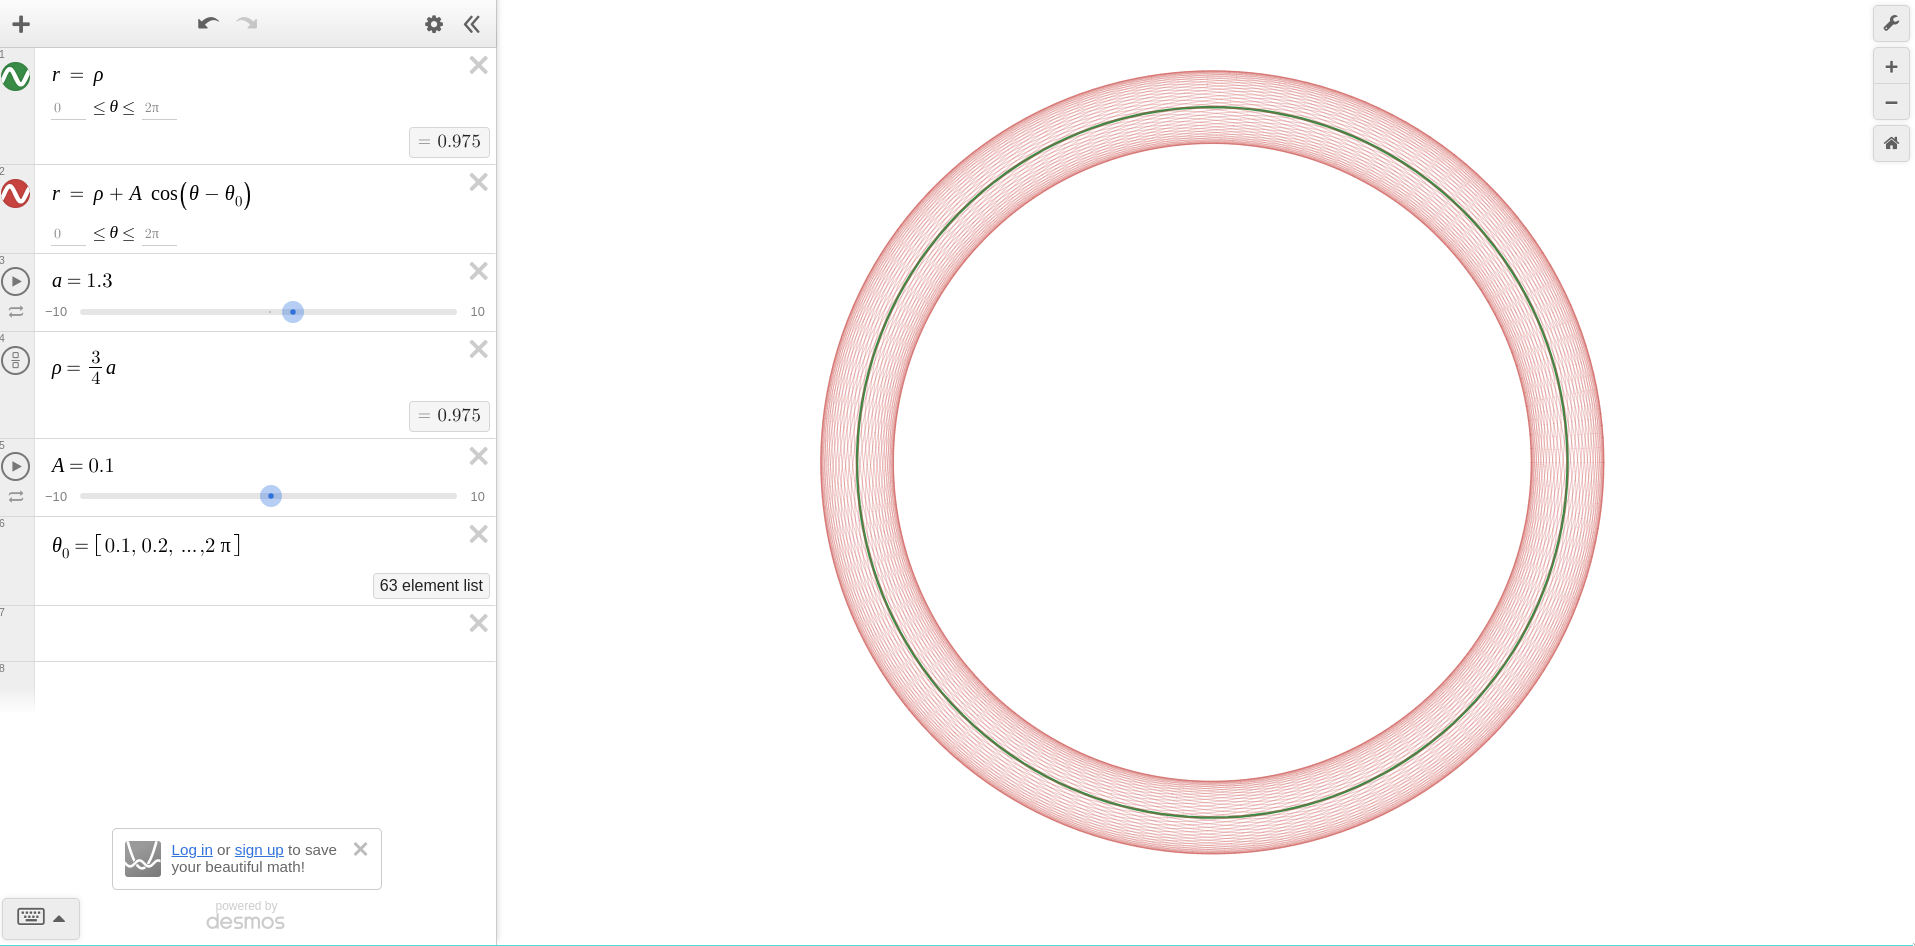
\includegraphics[width=0.8\textwidth]{./ss/8/1.png}
	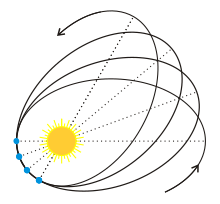
\includegraphics[width=0.4\textwidth]{./ss/8/2.png}
	\caption{./ss/8/1.png}
	\label{fig:-ss-8-1-png}
\end{figure}

\section*{Problem 02} 
The position of the particle in terms of $(r,\theta, \phi)$ where $r = r(t)$ is a given function of time, the generalized coordinates can be $\theta = \theta(t) = q_\theta(t)$ and $\phi = \phi(t) = q_\phi(t)$. 

\subsection*{(a)} 
\[
\mathcal L 
=
\frac{m}{2} \left(
r(t)^2 \dot{\theta}^2 + 
r(t)^2 \sin ^2 \theta \dot{\phi}^2
\right)
- 
mg r (t) \cos \theta 
\] 
\begin{align*}
	\mathcal H &= \sum_{n=1}^{2} \dot q_n \frac{\partial \mathcal L}{\partial \dot{q}_n} - \mathcal L  
		\\ &=
\dot{\theta} \frac{\partial \mathcal L}{\partial \dot{\theta}} + 
\dot{\phi} \frac{\partial \mathcal L}{\partial \dot{\phi } } - \mathcal L
	\\
&= \frac{m}{2} \left[\dot{\theta} \left(2 \dot{\theta} r^2(t)\right)  + 
\dot{\phi}
\left(2
\dot{\phi} r^2(t) \sin ^2 \theta 
\right)\right] - 
\frac{m}{2} \left(
r(t)^2 \dot{\theta}^2 + 
r(t)^2 \sin ^2 \theta \dot{\phi}^2
\right)
+ 
mg r (t) \cos \theta 
\\
&= \frac{m}{2} \left[ \left(2 \dot{\theta}^2 r^2(t)\right)  + 
\left(2
\dot{\phi}^2 r^2(t) \sin ^2 \theta 
\right)\right] - 
\frac{m}{2} \left(
r(t)^2 \dot{\theta}^2 + 
r(t)^2 \sin ^2 \theta \dot{\phi}^2
\right)
+ 
mg r (t) \cos \theta 
\\
&= \frac{m}{2} \left(
r(t)^2 \dot{\theta}^2 + 
r(t)^2 \sin ^2 \theta \dot{\phi}^2
\right)
+ 
mg r (t) \cos \theta  = E(t)
\\
\end{align*}



\subsection*{(b)}
Solving for the generalized momentum 
\begin{align*}
	p_n &= \frac{\partial \mathcal L}{\partial \dot q_n}\\  \ \\
	p_\theta &= m r^2(t) \dot{\theta}  \\ 
	p_\phi &= m \dot{\phi}^2 r^2 (t) \sin ^2 \theta  
\end{align*}
Solving for derivatives of generalized momentum 
\begin{align*}
	\dot{p}_n &= -  \frac{\partial \mathcal \mathcal H}{\partial q_n}  \\ \ \\
	\dot{p}_\theta &= m g r(t) \sin \theta - m r^2(t) \dot{\phi}^2 \sin \theta \cos \theta  \\  
	\dot{p}_\phi &= 0 
\end{align*}

Writing the Hamiltonian in terms of new variables 
\[
\mathcal H = 
\frac{p_\theta ^2}{2 m r^2 (t)} + 
\frac{p^2_\phi}{2 m r^2(t) \sin ^2 \theta} -
\frac{1}{2} m \dot{r}^2(t) + mg r(t) \cos \theta
\] 

\subsection*{(c)} 
We can see that the Hamiltonian is equal to the total energy $T + V$. The constraints working here (constraint of sphere until in contact) is time independent, forces here are conservative - hence it makes sense. 

There is a time dependence on one of the coordinate variables $r(t)$ which makes the system NOT to be conserving energy. 




\section*{Problem 03}
Position representation \[
	\vec{r} = \rho \hat{\rho} + z \hat{e}_z
\] 
Velocity representation \[
	\vec{v} = \dot{\vec{r}} = \dot{\rho} \hat{\rho} + r \dot{\theta} \hat{e}_\theta + 
	\dot{z} \hat{e}_z
\]

\begin{align*}
	|\vec{r}|^2 &= \rho^2 + z^2 \\
	(\vec{r} \cdot \hat{e}_z) &= z \\
	\vec{\omega} \times \vec{r} &= \rho \omega \hat{\phi}  \\
\end{align*}


\subsection*{(a)} 
\[\boxed{
\mathcal L 
=
\frac{1}{2} m (\dot{\rho } ^2 + \rho ^2 \dot{\phi}^2 + \dot{z}^2 ) + 
\frac{1}{4} m \Omega^2 (\rho^2 - 2 z^2) 
- \frac{1}{2} m \rho^2 \dot{\phi} \omega  
\tag{$\omega = e B  / m c $ }}
\] 

\subsection*{(b)} 
\begin{align*}
	p_\rho &= \frac{\partial \mathcal L}{\partial \dot{q}_\rho } 
	= m \dot{\rho} 
	       & \dot{\rho} &= \frac{P_\rho}{m} \\ 
	p_\phi &= \frac{\partial \mathcal L}{\partial \dot{q}_\phi}
	= m \rho^2 \dot{\phi} - \frac{1}{2} m \rho^2 \omega 
	       & \dot{\phi} &= \frac{p_\phi + \frac{1}{2} m \rho^2 \omega }{m \rho^2}\\
	p_z &= \frac{\partial \mathcal L}{\partial \dot{z} } = m \dot{z}
	    & \dot{z} &= \frac{p_z}{m} \\
\end{align*}
Using the equation of Hamiltonian I solve
\[
\mathcal H 
= 
p_\rho \dot{\rho} + 
p_\phi \dot{\phi} + 
p_z \dot{z} - L
\] 
\[
\boxed{
\mathcal H 
=
\frac{p_\rho ^2}{m} + 
\frac{p^2_\phi}{2 m \rho} + 
\frac{p_z^2}{2m} + 
\frac{\omega}{2} p_\phi + 
\frac{1}{8} m \left(\omega^2 - 2 \Omega^2\right) \rho^2
+ 
\frac{1}{2} m \Omega^2 z^2
}
\] 

\subsection*{(c)}
\begin{align*}
	\dot{\rho} &= \frac{\partial \mathcal H}{\partial p_\rho} = \frac{p_\rho}{m} 
		   & \dot{p_\rho} &= - \frac{\partial \mathcal H}{\partial \rho}
		   = \frac{1}{4} m (\omega^2 - 2 \Omega^2) \rho \\
	\dot{\phi} &= \frac{\partial \mathcal H}{\partial p_\phi} = \frac{p_\phi}{m \rho} + \frac{\omega}{2}
		   & \dot{p}_\phi &= - \frac{\partial \mathcal H}{\partial \phi} = 0 \\
	\dot{{z}} &= \frac{\partial \mathcal H}{\partial p_z} = \frac{p_z}{m} 
		  & \dot{p}_z &= - \frac{\partial \mathcal H}{\partial z} = - m \Omega^2 z
\end{align*}
Note that for the $z$ motion we have 
\[
\ddot{z} + \Omega^2 z = 0
\] 
The $z$ motion is a simple harmonic oscillator with $\Omega$ frequency. $\Omega$ is important because it characterizes the effective entrapment of the particle in $z$ axis.


\subsection*{(d)} 
Because 
\[
\dot{p}_\phi = \frac{\partial \mathcal H}{\partial \phi} = 0 \implies p_\phi = \text{const}
\] 
$\phi$ is a cyclic coordinate. 
\[
\dot{\phi} = \frac{p_\phi}{m \rho} + \frac{\omega}{2}
\]



\subsection*{(e)}
\begin{align*}
	\ddot{\rho} &= \frac{\dot p_\rho}{m} &\ddot{\rho}&=\frac{1}{m}
	\left(\frac{p_\phi^2}{m \rho^3 } - \frac{1}{4} m \left(\omega^2 - 2 \Omega^2\right)\rho\right)\\
		    & & 
	\ddot{\rho} &= 
\frac{p_\phi^2}{m^2 \rho^3 } - \frac{1}{4}  \left(\omega^2 - 2 \Omega^2\right)\rho \\
\end{align*}


\begin{align*}
	m \ddot{\rho} &= - \frac{\mathrm{d} U_\text{eff}}{\mathrm{d} \rho} \\ 
	U_\text{eff} (\rho) &= \int_{}^{} \mathrm{d} \rho \left(
\frac{p_\phi^2}{m^2 \rho^3 } - \frac{1}{4}  \left(\omega^2 - 2 \Omega^2\right)\rho 
	\right)
	\\
	U_\text{eff}(\rho)		    &=
			    \frac{p_\phi^2}{2 m \rho^2} + \frac{1}{8} m \left(\omega^2 - 2 \Omega^2\right) \rho ^2
\end{align*}

Plotting, $U_\text{eff} (x)= \frac{a}{x^2} + b x^2 $
$a$ is always greater than $0$. $b < 0$ when $\omega^2 - 2 \Omega^2 < 0 \implies \omega < \sqrt{2}  \Omega$ we have the following plot. 
\begin{figure}[H]
	\centering
	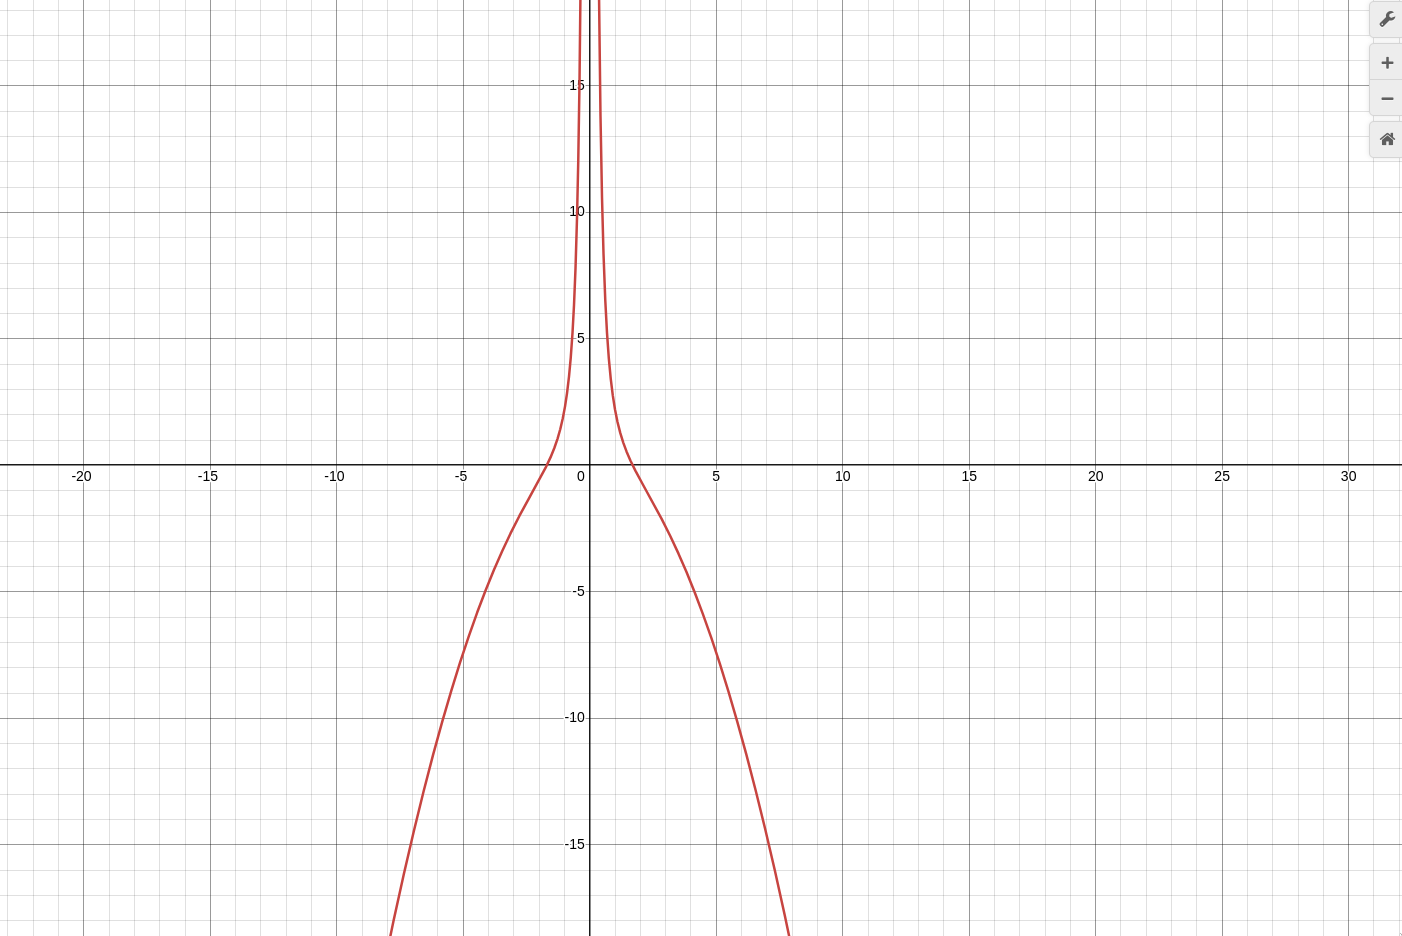
\includegraphics[width=0.8\textwidth]{./ss/8/3.png}
	\caption{./ss/8/3.png}
	\label{fig:-ss-8-3-png}
\end{figure}
When $\omega^2 - 2 \Omega^2 > 0 \implies \omega > \sqrt{2} \Omega$ that means $b>0$ we have 
\begin{figure}[H]
	\centering
	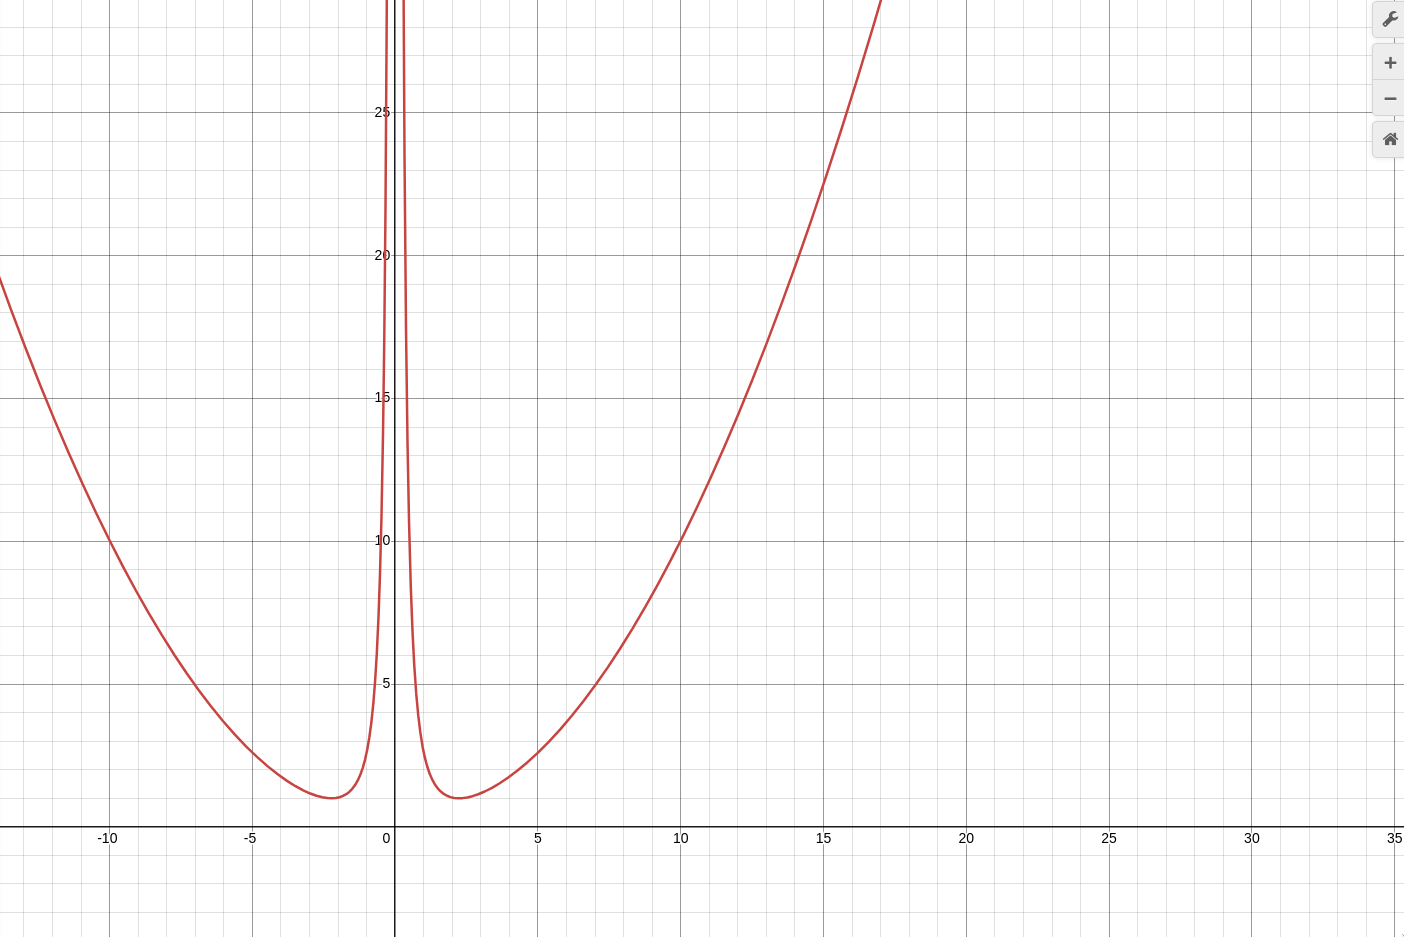
\includegraphics[width=0.8\textwidth]{./ss/8/4.png}
	\caption{./ss/8/4.png}
	\label{fig:-ss-8-4-png}
\end{figure}

\section*{Problem 04} 
The speed gained from the impulse adds to the radial component of the overall velocity. That speed $v_r$ is given by 
\[
m v_r = {I}\implies v_r = \frac{I}{m}
\]
The tangential speed already is 
\[
	v_t ^2 = \frac{GM}{r_0} = \frac{k}{mr_0 }
\] 


\subsection*{(a)} 
The orbit initially before impulse is a circular orbit with distance from the center being $r_0$. The velocity is $v_t$. 

When the impulse has been applied, we now have a velocity $\vec{v} = v_t \hat{\theta} - v_r \hat{r}$, at a distance $r_0$ from the ``center" (which is now a focus of the orbit). We know there must exist an elliptical orbit that keeps the old center in the focus and satisfies the following speed - position relation 
\[
v^2 = GM \left(\frac{2}{r} - \frac{1}{a}\right)
\] where $a$ is the semi-major axis. 

Solving for $a$ would give us helpful information about the geometry of the orbit. Right after the impulse, 

\begin{align*}
	v^2 &= \frac{k}{m}\left(\frac{2}{r_0} - \frac{1}{a}\right) \\ 
	\frac{k}{mr_0} + \frac{I^2}{m^2} &= \frac{k}{m} \left(\frac{2}{r_0} - \frac{1}{a}\right)
	\\
	\frac{1}{r_0} + \frac{I^2}{k m} &=  \left(\frac{2}{r_0} - \frac{1}{a}\right) 
	\\
	\frac{I^2}{m k} &= \frac{1}{r_0} - \frac{1}{a}
\\ 	
\frac{1}{a} &= \frac{1}{r_0} - \frac{I^2}{  m k } \\
a &= \frac{1}{ \frac{1}{r_0} - \frac{I^2}{m k}}
\end{align*}
We have solved for $a$ being
\[
a = \frac{1}{ \dfrac{1}{r_0} - \dfrac{I^2}{m k}}
\] 
The eccentricity is given by 
\[
\varepsilon = 
\sqrt{1 + 2 \frac{E L^2}{m k ^2}} 
\]
The energy here is 
\[E = 
	- \frac{1}{2} \frac{GM m }{r_0} + \frac{1}{2}m v_r^2 = 
	- \frac{1}{2} \frac{GM m }{r_0} + \frac{1}{2}m \frac{I^2}{m^2} 
= \frac{I^2}{2m}- \frac{k}{2 r_0} 
\implies \frac{1}{2} \left(\frac{I^2}{m}- \frac{k}{ r_0} \right)
\] 
The angular momentum here is 
\[
L^2 = m^2 v_t^2 r_0^2 = m^2 \frac{k}{m r_0} r_0^2 = m k r_0
\] 
Plug them in and solve for $\varepsilon$
\begin{align*}
	\varepsilon &= 
\sqrt{1 + 2 \frac{E L^2}{m k ^2}}  \\ 
&= \sqrt{1 + \frac{2}{m k  ^2} \frac{1}{2} \left(\frac{I^2}{m} - \frac{k}{r_0} \right) \left( m k  r_0\right)}   \\
&= \sqrt{1 + \frac{1}{m k  ^2}  \left({I^2}k r_0 -  m k^2  \right) }  \\
&= \sqrt{1 +   \left(\frac{I^2 r_0}{m k}-  1  \right)  } \\
&= \sqrt{\frac{I^2 r_0}{m k}  }  = 
I \sqrt{\frac{r_0}{ m k}} 
\end{align*}

The relation between Semi-Minor axis $b$, Semi-Major axis $a$, and Semi-Latus Rectum $\ell $
\begin{align*}
	b &= a \sqrt{1 - \varepsilon^2} 
	\\
	\ell &= a(1 - \varepsilon^2)
\end{align*}
Computing the Semi-Latus Rectum $\ell$
\[
\ell = \frac{r_0}{\frac{1}{r_0} - \frac{I^2}{m k }} \left(
\frac{1}{r_0} - \frac{I^2}{ m k} \right) = r_0
\] 

\[
\boxed{
\varepsilon = 
I \sqrt{\frac{r_0}{m k }} 
}
\] 
\[
\boxed{
\ell = r_0
}
\] 



\subsection*{(b)} 
\begin{figure}[H]
	\centering
	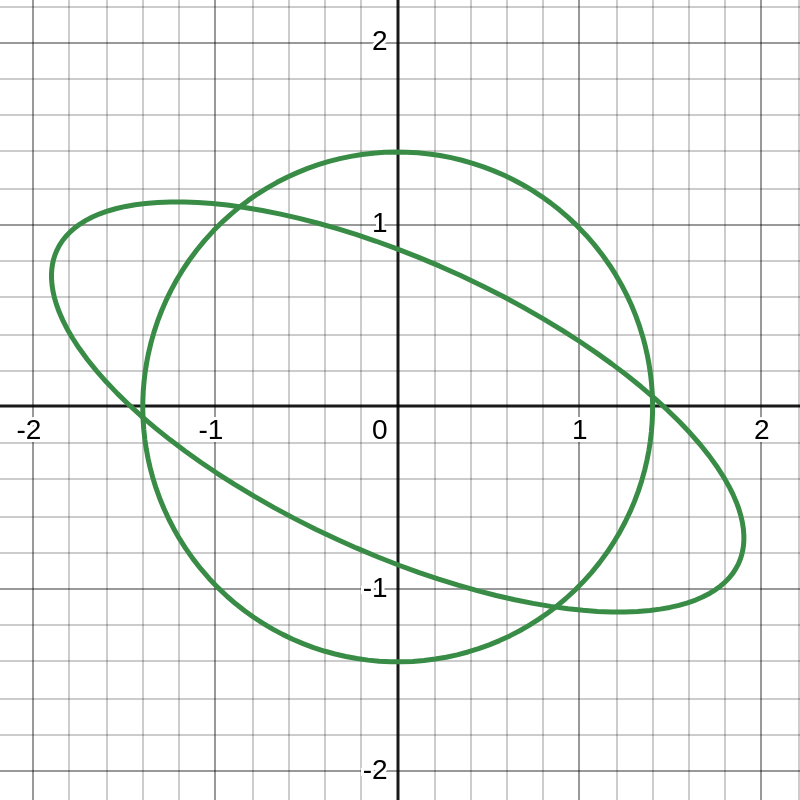
\includegraphics[width=0.8\textwidth]{./ss/8/5.png}
	\caption{Inward impulse and outward impulse will have similar orbit shapes.}
	\label{fig:-ss-8-5-png}
\end{figure}
If there's an \textbf{inward impulse}, then assuming there's a \textbf{counter clockwise} moving orbit, the ellipse intersection with circle orbit is going to be (where transition happens) will be in 1st Quadrant, 3rd Quadrant (when ellipse is intersecting \textbf{into} the circular orbit). 

Outward impulse is easy to understand, for this case it's the 2nd and 4th quadrant of coordinate system intersection. Ellipse is intersection \textbf{out} of the circular orbit.


\subsection*{(c)} 
\begin{align*}
	\overline{F} &= \frac{1}{T} \int_{0}^{T} \frac{1}{r^2} \, \mathrm{d} t  \\
	E &= - \frac{GM}{2a} \\
	\frac{I^2}{2m^2} - \frac{GM}{2 r_0} &= - \frac{GM}{2a} 
\end{align*}
\[
\boxed{
\frac{1}{a} = \frac{1}{r_0} - \frac{I^2}{6Mm^2}
}
\] 
The manuever is counterproductive because $a$ increases if it was going towards the star. The impulse should be applied away from the star to decrease $a$.




\section*{Last Homework: Problem 05} 
\subsection*{(a)} 
The cross product $\mu r \hat{\phi}$. Hence
\[
\boxed{
	\frac{1}{2} m 
	\left(\dot \rho ^2 + \rho ^2 \dot{\phi}^2 + \dot{z}^2\right) + \frac{q \mu \rho^2 \dot{\phi}}{(\rho^2 + z^2)^{\frac{3}{2}}}
}
\] 


\subsection*{(b)} 
\begin{align*}
	p_\rho &= \frac{\partial L}{\partial \dot\rho} = m \dot{\rho} 
	       & \dot{\rho} &= \frac{p_\rho}{m} \\ 
	p_\phi &= \frac{\partial L}{\partial \dot{ \phi} } = m \rho^2 \dot{\phi}  + \frac{q \mu \rho^2}{(\rho^2 + z^2)^{\frac{3}{2}}} 
	       & \dot{\phi} &=  \frac{1}{m \rho^2 } \left(\rho_\phi - \frac{q \mu \rho^2 }{(\rho^2 + z^2)^{\frac{3}{2}}}\right)\\
	p_z &= \frac{\partial L}{\partial \dot{z}} = m \dot{z} 
	    &\dot{z} &= \frac{p_z}{m} 
\end{align*}
I did this following computation on paper. What I got. \[
\boxed{
\mathcal H = \frac{p_\rho^2}{2m} + \frac{p_z^2}{2m} + \frac{1}{2m \rho^2} 
\left(
p_\phi - \frac{q \mu \rho^2}{(\rho^2 + z^2)^{\frac{3}{2}}}
\right)^2
}
\] 

\subsection*{(c)} 
$H=E$, yes the hamiltonian is equal to the total energy $E$. There is no explicit time dependence so energy is conserved.


\subsection*{(d)}
Hamiltonian doesn't depend explicitly on $\phi$ so $\phi$ is a cyclic coordinate. Therefore
\[
\ell = p_\phi = m \rho^2 \dot{\phi} + \frac{q \mu \rho^2}{(\rho^2 + z^2)^{3 / 2}}
\] 


\subsection*{(e)} 
\begin{align*}
	\dot{\rho} &= \frac{p_\rho}{m} \\ 
	\dot{p_\rho} &= \frac{1}{m \rho^3} 
	\left( p_\phi - \frac{q \mu \rho^2}{r^3}\right)^2 
	- 
	\frac{1}{m \rho^2}
	\left(
2 
\left[
p_\phi - \frac{q \mu \rho^2}{r^3}  
\right]
\left[
- 2 \frac{q \mu \rho}{r^3} 
+
3 \frac{q \mu \rho^3}{r^{5}}
\right]
	\right)\\
	\dot{z} &= \frac{p_z}{m} \\
	\dot{p_z} &= - \frac{2}{m \rho^2} \left(p_\phi - \frac{q \mu \rho^2}{r^3} \right)
	\left(3 \frac{q \mu \rho^2 z}{r^{5}}\right)\\
\end{align*}


\subsection*{(f)}
\[
\boxed{
E = \frac{p_\rho ^2}{2m} + \frac{1}{2m} \left(
\frac{p_\phi}{\rho} - \frac{q \mu }{\rho^2}
\right)
}
\] 
\begin{figure}[H]
	\centering
	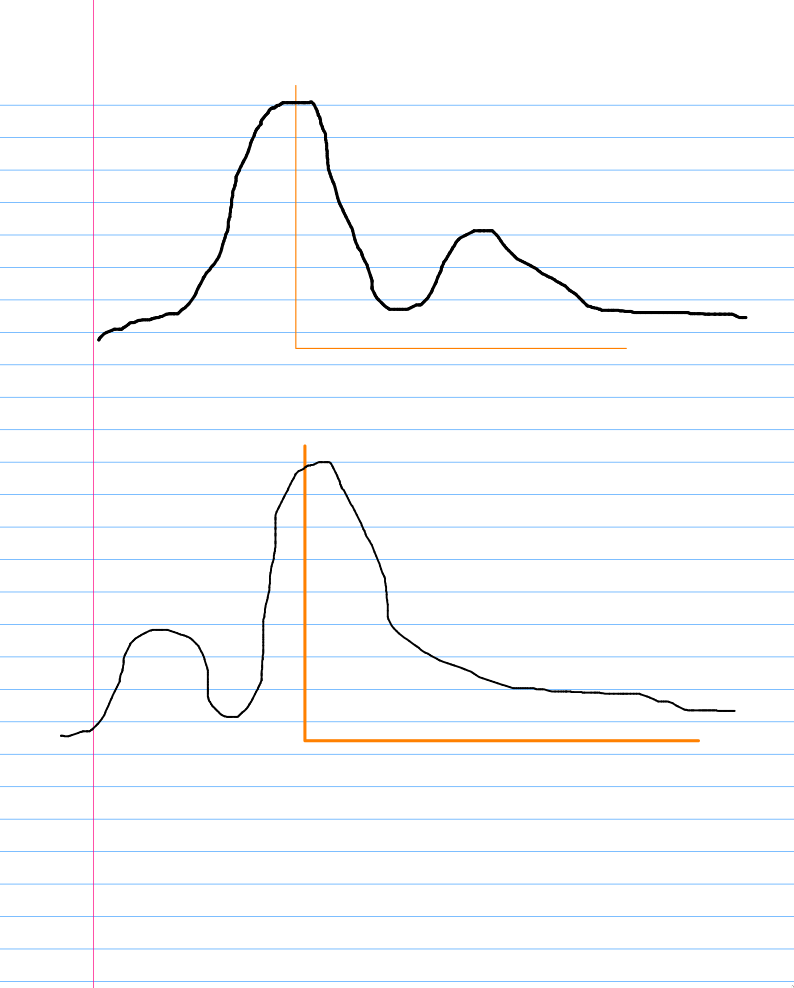
\includegraphics[width=0.8\textwidth]{./ss/8/6.png}
	\caption{./ss/8/6.png}
	\label{fig:-ss-8-6-png}
\end{figure}
\end{document}
